\documentclass{article}
\usepackage[utf8]{inputenc}

\usepackage[backend=bibtex]{biblatex}
\addbibresource{dmu-gnn.bib}
% \usepackage{indentfirst}
\usepackage{hyperref}
\usepackage[a4paper, total={6in, 10in}]{geometry}
\usepackage{amsmath}
\usepackage{graphicx}
\usepackage[utf8]{inputenc} % allow utf-8 input
\usepackage[T1]{fontenc}    % use 8-bit T1 fonts
\usepackage{hyperref}       % hyperlinks
\usepackage{url}            % simple URL typesetting
\usepackage{booktabs}       % professional-quality tables
\usepackage{amsfonts}       % blackboard math symbols
\usepackage{nicefrac}       % compact symbols for 1/2, etc.
\usepackage{microtype}      % microtypography
\usepackage{xcolor}         % colors
\usepackage{float}
\setlength{\parindent}{0pt}

\title{% 
    Automated Theorem Proving with Graph Neural Networks}
\author{Daniel Jenson, Daniel Huang and Julian Cooper}
% \date{January 20th, 2023}

\begin{document}

\maketitle

% Requirements: You will provide a 1 page status update partway into the quarter. Please re-introduce the problem, outline what you have been able to accomplish, and provide a revised timeline to completion. Please have ONE group member submit your status update on Gradescope.


\vspace{-3em}
% Re-introduction 
\section{Problem Statement}
Theorem proving is a difficult, lengthy process, which has historically been the sole employ of mathematicians. Recent engineering and computer science advances have seen the advent of theorem proving assistants. These are software programs that aid mathematicians in proving statements by providing a formal syntax for composing proofs and a verification process for validating them. More recently, some of these software programs have begun to provide automated theorem proving (ATP) components, which are capable of automatically selecting tactics and proving simpler sub-goals. Since 2019, these ATP modules have been further augmented with neural networks, creating a new class of ATPs called Neural Theorem Provers (NTPs). NTPs are often structured as an encoder-decoder, which consists of an encoder embeds goals in a latent space and a decoder that uses these representations to produce a distribution over the tactics. In this project, we attempt to extend one of these NTP frameworks.

\begin{figure}[h]
    \centering
    % Kind of small for coq architecture, not sure if that matters much
    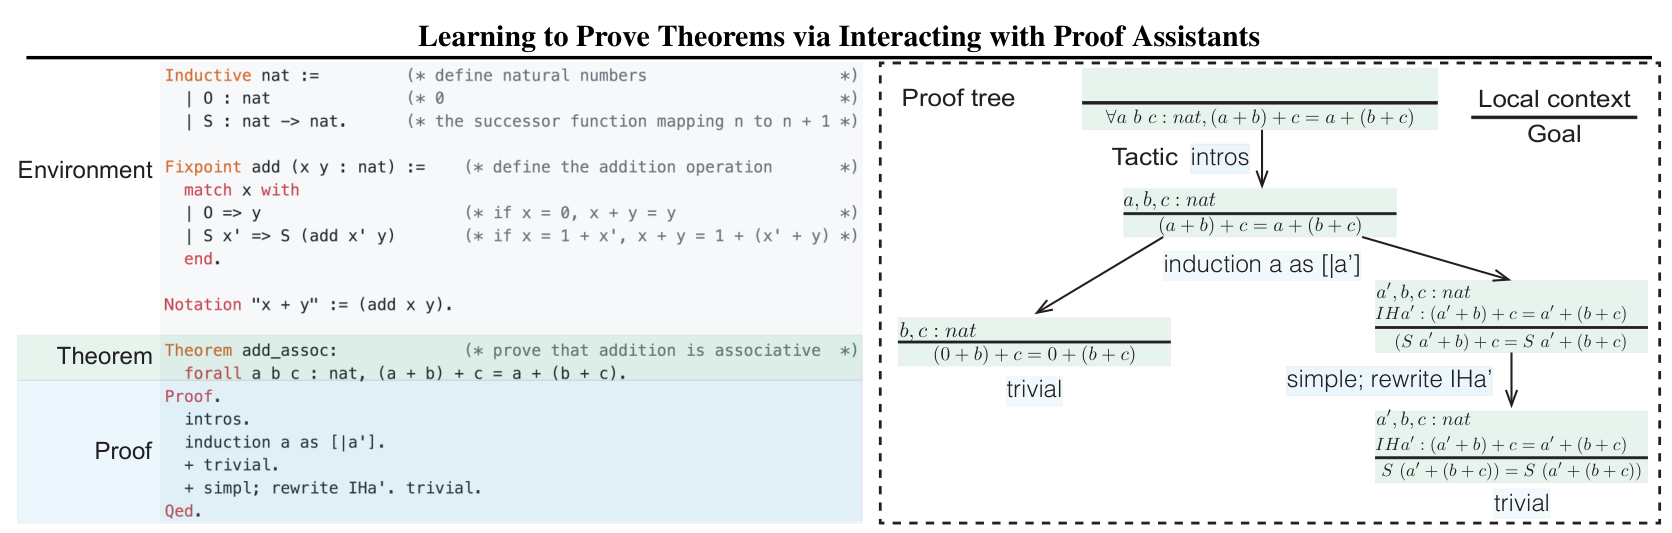
\includegraphics[width=0.9\textwidth]{images/proof_assistant_example.png}
    \caption{Automated Proof Assistant: example for induction "tactic" \cite{coqgym}}
    \label{fig:atp}
\end{figure}

There are two principle baselines: CoqGym and HOList. CoqGym is based on the Coq theorem proving language and HOList is based on the HOL Light theorem prover. For this project, we elected to use Coq, since it had open source data and code. (The HOList team at Google did end up sending us data but could not open source parts of their codebase). The NTP for our project is composed of two parts: (1) the encoder-decoder and (2) the reinforcement learning agent. The encoder-decoder is a neural network that is trained with teacher forcing using human proofs. At test time, the reinforcement learning agent uses the output of the encoder-decoder and applies estimated high value tactics to the current goal. It limits the number of tactic applications to 300 or 10 minutes of runtime. It is rewarded when a goal and all of its subgoals are proved. Below, we provide the details on our progress and next steps.

\section{Progress}
% (1) Worked with CoqGym maintainers to reproduce their training and testing pipeline locally. (2) Setup on CS server with same pipeline to enable future parallel training. (3) Drafted GNN that runs locally but is not yet parallelised / gpu enabled so the complete run.

Over the past couple of weeks, we made significant progress on reproducing CoqGym pipelines and some implementations: 

\begin{enumerate}
    \item \textbf{Reproduced CoqGym training and testing pipelines locally}: The installation process is very complex, requiring the installation of OCaml and a variety of packages, the compilation of a custom version of the Coq theorem proving software, the extraction of proofs from the Coq language to ASTs that can be manipulated in Python, and the compilation of other external theorem proving agents called ``hammers.'' This process requires approximately 12 hours of computation and 55 GB of storage. We also had to submit several fixes and improvements to this process, since the existing code was broken or underspecificied (e.g. missing pytorch version). After completing this, we also realized that training these models locally was prohibitive, so we repeated this process on 3 different servers so we could run multiple experiments.
    \item \textbf{Parallelized proof extraction script}: The proofs dataset needs to be processed into individual \texttt{.pickle} files. The script they provided worked in series, but the process was very slow. Since this was trivially parallelizable, we wrote a script to speed this up from approximately 12 hours to around 4.
    \item \textbf{Integrated an unoptimized GNN in place of the TreeLSTM}: The \texttt{CoqGym} paper \cite{coqgym} implemented a TreeLSTM term encoder. We expect to improve upon this with a Graph Neural Network, configured similarly to the encoder proposed in Google's HOList paper \cite{hol}, but adding in components such as Differential Pooling\cite{hier} which improve the extraction process. Currently, our draft implementation of the GNN uses two graph convolution layers (2-hop) and max-pooling aggregation. 
\end{enumerate}

\begin{figure}[H]
    \centering
    % Kind of small for coq architecture, not sure if that matters much
    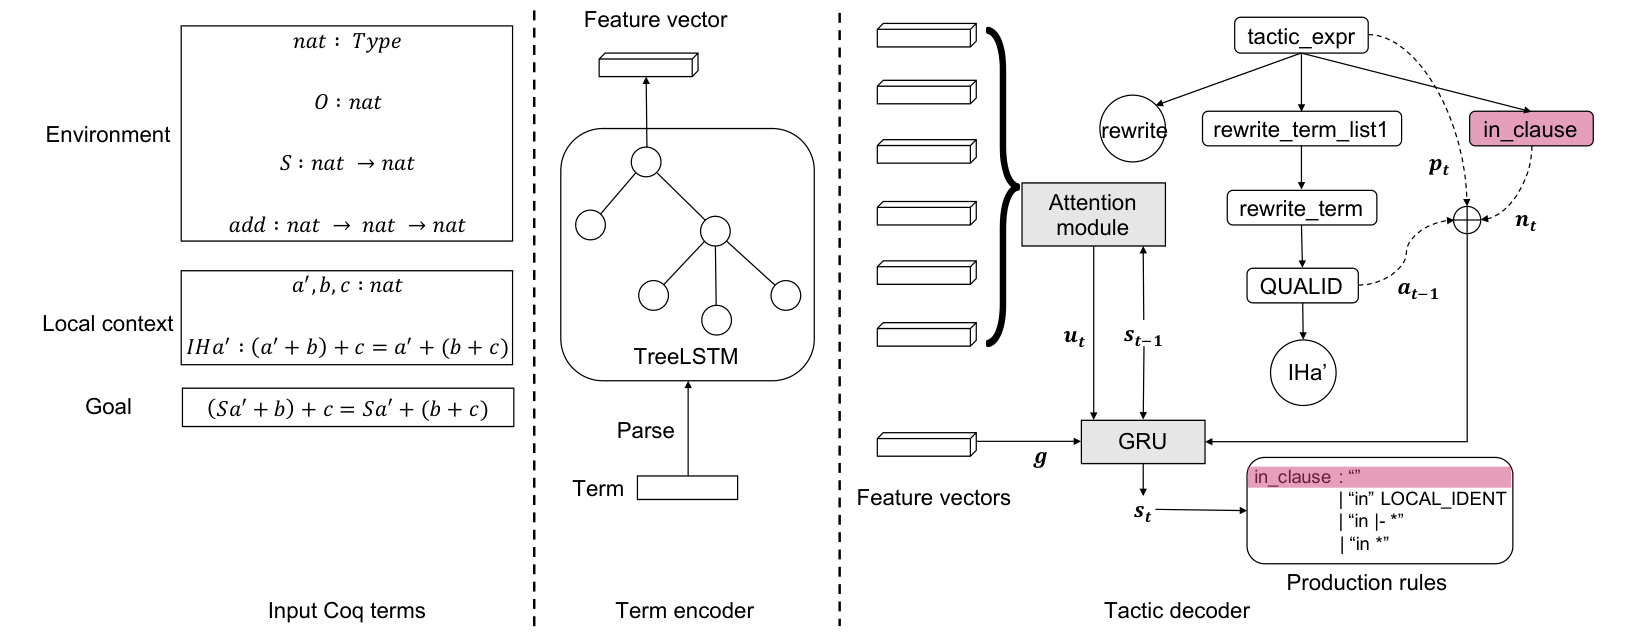
\includegraphics[width=1\textwidth]{images/coqgym.png}
    \caption{CoqGym model architecture \cite{coqgym}}
    \label{fig:coq_arch}
\end{figure}


\section{Timeline \& next steps}
% Implement modifications to GRU? 
Now we have a working end-to-end pipeline, our goal for the remainder of this project is to reproduce the \texttt{CoqGym} benchmarks and implement two extensions:
\begin{itemize}
    \item \textbf{Reproduce \texttt{CoqGym} benchmarks}: While we have the \texttt{CoqGym} pipeline up and running and are able to reproduce their testing results for a single proof, we have not been able to run for all test proofs. We need to do this to confirm we can reproduce their benchmarks before comparing with our extensions.
    
    \item \textbf{Improve and tune GNN term encoder}: Two major improvements we have planned: (1) enable the GNN to make use of multiprocessing to speed up training on our remote server, and (2) utilize differential pooling (a more expressive, recently development technique) instead of max-pooling for aggregation \cite{hier}.
    
    \item \textbf{Calibrate reinforcement agent}: The agent described in the \texttt{CoqGym} paper \cite{coqgym} is relatively simple: the agent passes the goal and context to the encoder-decoder, learns the probability distribution over available tactics, and sends the top 300 of these to the prover (environment) and receives subgoals (states) from the prover. We want to experiment with getting our agent to make smarter decisions about (a) which tactics to select from the distribution outputs from the encoder-decoder and (b) when it is appropriate to step back in the proof tree (delete a node). To do this, our first step is to create a SARSA dataset and use this to tackle the problem in isolation (outside of such a large pipleine) with different model-free solver techniques learned from class (e.g. q-learning).

\end{itemize}

We hope these extensions will generate results that improve upon \texttt{CoqGym}'s benchmark of ~30\% for its automated theorem prover (ASTactic + Hammer)!

\end{document}
